\begin{figure}[H]
\scalebox{0.5}{%
    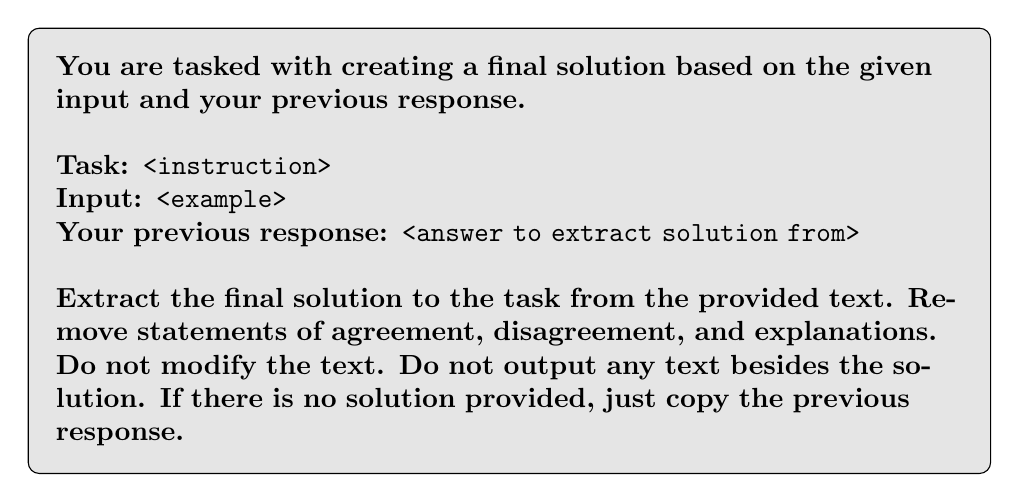
\begin{tikzpicture}
    \node [draw, rectangle, rounded corners, fill=gray!20, text width=0.95\textwidth, inner sep=10pt] (block) {
        \begin{minipage}{\textwidth}
        \textbf{You are tasked with creating a final solution based on the given input and your previous response.} \\
        
        \textbf{Task:} \texttt{<instruction>} \\
        \textbf{Input:} \texttt{<example>} \\
        \textbf{Your previous response:} \texttt{<answer to extract solution from>} \\
        
        \textbf{Extract the final solution to the task from the provided text. Remove statements of agreement, disagreement, and explanations. Do not modify the text. Do not output any text besides the solution. If there is no solution provided, just copy the previous response.}
        \end{minipage}
    };
    \end{tikzpicture}
}
\caption{Prompt to extract the solution from an agent's answer.}
\end{figure}
